\documentclass[tikz]{standalone}
\RequirePackage{fontspec}
\IfFontExistsTF{calibri.ttf}
{
  \setmainfont{calibri.ttf}[
    BoldFont = calibrib.ttf,
    ItalicFont = calibrii.ttf,
    BoldItalicFont = calibriz.ttf
  ]
}
{}
\usetikzlibrary{arrows.meta}

\definecolor{one}{RGB}{255, 192, 110}
\definecolor{two}{RGB}{123, 116, 255}
% \usepackage{times}
\definecolor{bg}{RGB}{40, 44, 52}
\definecolor{text}{RGB}{86, 182, 194}

% \pagecolor{bg}
\begin{document}

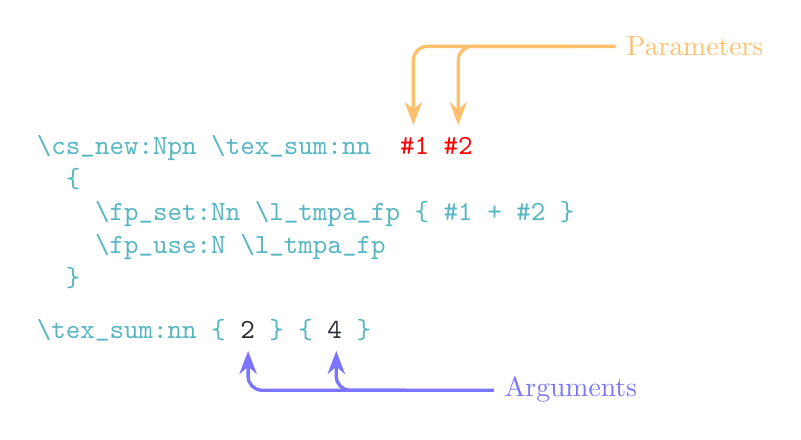
\begin{tikzpicture}
    \node[font = \ttfamily, text = text, align = left, anchor = west] (a) at (0,0) 
    {
        \verb|\cs_new:Npn \tex_sum:nn| \color{red}\verb| #1 #2| \\
        \verb|  {| \\
        \verb|    \fp_set:Nn \l_tmpa_fp { #1 + #2 }| \\
        \verb|    \fp_use:N \l_tmpa_fp| \\
        \verb|  }|
    };

    \node[font = \ttfamily, text = text, align = left, anchor = west] (b) at (0,-1.5) 
    {
        \verb|\tex_sum:nn { |{\color{bg}\verb|2|} \verb|}|\verb| { |{\color{bg}4}\verb| }|
    };
    \draw[rounded corners = 5pt, Stealth-, very thick = 1pt, one] ([xshift = -2.17cm]a.north east) |- ++ (2, 1);
    \draw[rounded corners = 5pt, Stealth-, very thick = 1pt, one] ([xshift = -1.6cm]a.north east) |- ++ (2, 1) node[anchor = west, text = one] {Parameters};

    \draw[rounded corners = 5pt, Stealth-, very thick = 1pt, two] ([xshift = -1.87cm]b.south east) |- ++ (2, -.5);
    \draw[rounded corners = 5pt, Stealth-, very thick = 1pt, two] ([xshift = -.75cm]b.south east) |- ++ (2, -.5)node[anchor = west, text = two] {Arguments};
\end{tikzpicture}
\end{document}